\section{Lezione del 09/05/2018}

\subsection{Programmazione Dinamica}

Da \href{https://it.wikipedia.org/wiki/Programmazione_dinamica}{Wikipedia}: 
\begin{quote}
    In Informatica la \emph{programmazione dinamica} è una tecnica di progettazione di algoritmi basata sulla divisione del problema in 
    sottoproblemi e sull'utilizzo di sottostrutture ottimali. 
\end{quote}

La programmazione dinamica è utilizzata in casi in cui i sottoproblemi vengono richiamati molte volte, rendendo
conveniente salvare in memoria il risultato di tali sottoproblemi per non doverli ricalcolare a ogni iterazione. Ad esempio, possiamo immaginare che i dati vengano
immagazzinati in una tabella:

\begin{center}
    \begin{tabular}{|c|c|c|}
        \hline
        $P_1$ & sol. $P_1$ & costo $P_1$ \\
        \hline 
        $P_2$ & sol. $P_2$ & costo $P_2$ \\
        \hline
        \dots & \dots & \dots \\
        \hline
    \end{tabular}    
\end{center}

\begin{enumerate}
    \item Caratterizzo la ``struttura'' della \emph{soluzione ottima} (soluzione ottima di $P$ in termini di soluzioni ottime di sottoproblemi);
    \item Espressione ricorsiva del \emph{valore} della soluzione ottima;
    \item Algoritmo che calcola il ``valore della soluzione ottima'':
    $$\Downarrow$$
    \[
        \begin{cases}
            \text{top down} \\
            \text{bottom up}
        \end{cases}
    \]
    \item Algoritmo che calcola la \emph{soluzione} e il \emph{valore}
\end{enumerate}

\subsubsection{Taglio delle aste}

Introduciamo la programmazione dinamica con un primo esempio. Ipotizziamo ci sia un'azienda che produce aste di metallo
molto lunghe, per venderle tagliate a pezzi.

Ogni pezzo ha un valore di vendita legato alla lunghezza. Voglio dei tagli che massimizzino il ricavo. Abbiamo
\begin{itemize}
    \item Lunghezza complessiva dell'asta $= n$;
    \item Prezzi $p_1, p_2, \dots , p_n$.
    \item $r_n$ Ricavo massimo ottenibile per l'asta di lunghezza $n$
\end{itemize}

\paragraph{Esempio} $n = 7$

\begin{center}
    \begin{tabular}{r|l|l|l|l|l|l|l}
        Lunghezza & 1 & 2 & 3 & 4 & 5 & 6 & 7 \\
        \hline
        $p_i$ & 1 & 5 & 8 & 9 & 10 & 17 & 17
    \end{tabular}
\end{center}
Come possiamo suddividere l'asta di lunghezza 7?

\begin{align*}
    \text{Suddivisione} & \rightarrow p_i \\
    1+1+ \dots +1 & \rightarrow 7 \\
    2+1+ \dots +1 & \rightarrow 10 \\
    2+2+2+1 & \rightarrow 16 \\
    7  & \rightarrow 17 \\
    6+1  & \rightarrow 18 \\
    2+2+3 & \rightarrow 18 \\
    \dots
\end{align*}
Sono possibili $2^{n-1}$ possibili combinazioni di tagli. È evidente che calcolarle tutte esplicitamente risulta estremamente inefficiente.

Supponiamo di tagliare l'asta in posizione $i$, tale che si ottenga una soluzione con due sottoproblemi ottimali (ottenendo le sotto-aste $a$ e $b$).

\begin{align*}
    r_n & = r_i + r_{n-i} \\
    r_n & = a + b \text{ con } a < r_i \\
    r_n' & = r_i + b > r_n \text{ (non ha particolare senso)} \\
    & i \text{ è ottimo?} \\
    r_0 & = 0 \\
    r_n & = max \left( \{ p_n \} \cup \{ r_i + r_{n-i} \ | \ i = 1 , \twodots, n-1 \} \right) \\
    & \qquad \text{($p_n$ non taglio, $r_{n-1}$ taglio, e ottimizzo le due parti)} \\
    & = max\{ p_i + r_{n-i} \ | \ i=1, \twodots, n \}
\end{align*}

\clearpage

\paragraph{Pseudocodice}
\begin{codebox}
    \Procname{$\proc{CutRod}(p,n)$}
\li \If $n = 0$
\li \Then \Return $0$
\li \Else
\li     $q \gets -1$
\li     \For $i = 1$ \To $n$
\li     \Do $q \gets \proc{Max}(q, P[i] + \proc{CutRod}(P,n-i))$ 
        \End
    \End
\li \Return $q$
\end{codebox}

\paragraph{Complessità}
\begin{align*}
    T(n) & = 1 + \displaystyle\sum_{i=1}^n T(n-i) \\
    & = 1 + \displaystyle\sum_{j=0}^{n-1} T(j) = \Theta(2^n) \\
    T(0) & = 1 + 0 = 1 = 2^0 \\
    T(n+1) & = 1 + \displaystyle\sum_{j=0}^n T(j) \\
    & = 1 + \displaystyle\sum_{j=0}^{n-1} T(n) + T(n) \qquad
    \left( \displaystyle\sum_{j=0}^{n-1} T(n) = T(n) \right) \\
    & = 2 T(n)
\end{align*}

\clearpage

Vediamo il problema della ripetizione dei sottoproblemi con $n = 4$
\begin{center}
    \begin{tikzpicture}
    \Tree
    [.$P4$
        [.${\color{red} P3}$
            [.${\color{green} P2}$ 
                [.${\color{blue} P1}$ 
                    [.${\color{cyan} P0}$ ]
                ]
                [.${\color{cyan} P0}$ ]
            ]
            [.${\color{blue} P1}$ 
                [.${\color{cyan} P0}$ ]
            ]
            [.${\color{cyan} P0}$ ]
        ]
        [.${\color{green} P2}$
            [.${\color{blue} P1}$ 
                [.${\color{cyan} P0}$ ]
            ]
            [.${\color{cyan} P0}$ ]
        ]
        [.${\color{blue} P1}$
            [.${\color{cyan} P0}$ ]
        ]
        [.${\color{cyan} P0}$ ]
    ]
    \end{tikzpicture}
\end{center}

Sfruttando la ``memoria'', restano i sottoproblemi risolti una sola volta:
\begin{center}
    \begin{tikzpicture}
    \Tree
    [.$P4$
        [.${\color{red} P3}$
            [.${\color{green} P2}$ 
                [.${\color{blue} P1}$ 
                    [.${\color{cyan} P0}$ ]
                    \edge[blank]; \node[blank]{};
                ]
                \edge[blank]; \node[blank]{};
            ]
            \edge[blank]; \node[blank]{};
        ]
        \edge[blank]; \node[blank]{};
    ]
    \end{tikzpicture}
\end{center}

\begin{itemize}
    \item \verb|#|sottoproblemi polinomiale ($n^k$) nella dimensione del problema di partenza;
    \item Esiste un algoritmo polinomiale per calcolare la soluzione del problema date le soluzioni dei sottoproblemi.
\end{itemize}

Sono possibili due approcci: 
\begin{itemize}
    \item Top-down con \emph{memoization};
    \item Bottom-up.
\end{itemize}

\paragraph{Top-down}
\begin{codebox}
    \Procname{$\proc{MemCutRod}(p,n)$}
\li \For $i \gets 1$ \To $n$
\li \Do $r[i] \gets -1$
    \End
\li \Return $\proc{MemCutRod}(p,n,r)$
\end{codebox}
\begin{codebox}
    \Procname{$\proc{MemCutRod-aux}(p,j,r)$}
\li \If $r[j] < 0$
\li \Then \If $j = 0$ 
\li     \Then $r[j] \gets 0$
\li     \Else 
\li         $q = -1$
\li         \For $i \gets 1$ \To $j$
\li         \Do $q \gets \proc{Max}(q, p[i]+\proc{MemCutRod-aux}(p,j-i,r))$
\li             $r[j] \gets q$
            \End
        \End
    \End
\li \Return $r[j]$
\end{codebox}

$$j = 1, \dots, n$$
\begin{gather*}
    \displaystyle\sum_{j=1}^{n} \left( \Theta(1) + j \Theta(1) \right) \\
    = \Theta \left( \displaystyle\sum_{j=1}^{n} (1+j) \right) = \Theta(n^2)
\end{gather*}

\paragraph{Bottom-Up}
\begin{codebox}
    \Procname{$\proc{BottomUpCutRod}(p,n)$}
\li $\text{alloco } r[1 \twodots n]$
\li $r[0] \gets 0$
\li \For $j \gets 1$ \To $n$ \Comment calcolo $r[j]$
\li \Do $q \gets -1$
\li     \For $i \gets 1$ \To $j$
\li     \Do $q \gets \proc{Max}(q, p[i] + r[j-1])$ \Comment $\Theta(1)$
        \End
        $r[j] \gets q$
    \End
\li \Return $r[n]$
\end{codebox}

$$\displaystyle\sum_{i=1}^n \displaystyle\sum_{i=1}^j \Theta(1) = \Theta (n^2)$$
